\subsection{Geometric Interpretation of Tangential Gradients} \label{ssec:3DGradGeometric}
Precise definition and analysis of the Sobolev spaces $\tgradSob{\ddom}{\dddmes}$ can be found in section \ref{sec:BorelMeasSobSpaces}, and explicit analysis of these spaces in section \ref{sec:3DGradSobSpaces}.
Our objective here is to provide the reader with an intuitive idea for the objects $\tgrad_{\ddmes}u$ and $\tgrad_{\dddmes}u$, and provide directs for the interested reader to the relevant analysis \tstk{add pointers to the results in the appendix when they are mentioned colloquially in this text}.

The intuition behind the form of the tangential gradients (and gradients of zero) with respect to the various measures $\lambda_{jk}, \ddmes, \massMes$, and $\dddmes$ can be summarised with the colloquial phrase ``tangential gradients only reflect behaviour that the measure can see".
Let us be more precise, and first consider the measure $\lambda_{jk}$ for a fixed $I_{jk}$ and the associated gradients of zero and tangential gradients.
Suppose that we have a (sufficiently smooth) function $u$ defined on $\ddom$ that satisfies $u=0$ (or any constant value) on $I_{jk}$; from the perspective of $\lambda_{jk}$ this $u$ is the zero function,\footnote{More precisely, $u$ is represented by the zero function in $\ltwo{\ddom}{\lambda_{jk}}$.} regardless of whether $u$ is zero on the whole of $\ddom$ or not.
So despite $u=0$ in $\ltwo{\ddom}{\lambda_{jk}}$, it can have any profile in the direction $n_{jk}$ \emph{as it crosses} $I_{jk}$ and thus any kind of (reasonable) behaviour in the rest of $\ddom$ --- this is schematically illustrated in figure \ref{fig:Diagram_GradZeroIllustrations}.
\begin{figure}[b!]
	\centering
	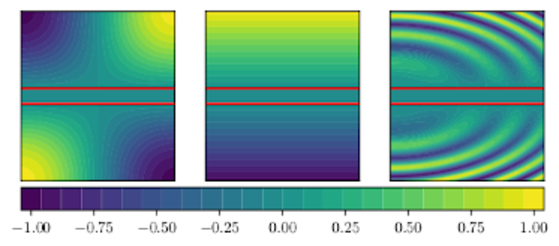
\includegraphics[scale=1.0]{Diagram_GradZeroIllustrations-Scaled.pdf}
	\caption{\label{fig:Diagram_GradZeroIllustrations} Examples illustrating how non-zero gradients of zero can arise, with the region between the red lines representing an edge $I_{jk}$, which has been thickened so one can view the function values along this edge. Despite each of the functions appearing constant along the edge $I_{jk}$, and thus constant to the measure $\lambda_{jk}$, the function is changing in the direction $n_{jk}$ as it crosses $I_{jk}$ and it's behaviour ``off the edge" is unknowable from the perspective of $\lambda_{jk}$.}
\end{figure}
Indeed, the measure $\lambda_{jk}$ is unable to deduce whether (for $x\in I_{jk}$) $u(x+hn_{jk})$ is different from $u(x)$ for $h\neq0$, given the only information it can have about $u$ are its values on $I_{jk}$.
Consequentially, the measure $\lambda_{jk}$ cannot bestow a concept of normal derivative $\pdiff{u}{n_{jk}}$ --- changing the profile of $u$ across the edge $I_{jk}$ does not change $u$ on $I_{jk}$.
Further to this, the component of any ``gradient" directed along $n_{jk}$ corresponds to no change in the function $u$ from the perspective of $\lambda_{jk}$.
A gradient that corresponds to no change in function must be (from our classical understanding) the gradient of a constant, or by our new understanding, a gradient of zero.
By contrast, the measure $\lambda_{jk}$ \emph{does} allows us to evaluate expressions like $u(x+he_{jk})-u(x)$ --- that is, we can detect changes in the function along $I_{jk}$.
Such changes correspond to $u$ changing in the direction tangential to the edge ($\pdiff{u}{e_{jk}}\neq 0$ classically), and thus we find that tangential gradients are directed along $e_{jk}$.
Since our singular measure is just the Lebesgue measure along $I_{jk}$, the tangential gradient possesses a classical derivative in this direction too.
This also highlights the reason for defining the gradients of zero and tangential gradients as in section \ref{sec:BorelMeasSobSpaces} --- given a tangential gradient $\ktgrad_{\lambda_{jk}}u$, $\lambda_{jk}$ can reconstruct the function $u$ along the edge $I_{jk}$, but cannot determine what $u$ is doing across $I_{jk}$.
Ergo, every function has a gradient that is unique up to a gradient of zero, because there is no way for $\lambda_{jk}$ to determine what $u$ looks like across (and thus outside of) $I_{jk}$.

The above story is similar when considering the tangential gradient of $u$ with respect to the measure $\massMes$.
Here, the ``view" of $\massMes$ is even more restricted than $\lambda_{jk}$, only being able to view the value of $u$ at the vertices, which are a set of isolated points in $\ddom$.
As such, there is no way for the measure $\massMes$ to reconstruct any kind of sensible gradient --- there are no ``nearby" function values $u\bracs{v_j + h x}, x\neq 0$ to compare the value of $u\bracs{v_j}$ to.
The result is corollary \ref{cory:NuTangGradChar}, any gradient must be a gradient of zero, because as far as $\massMes$ is concerned, there is no visible change in $u$ in any neighbourhood of $v_j$.
Then, given that $\dddmes$  is just the sum of the measures $\ddmes$ and $\massMes$, we find that $\tgrad_{\dddmes}u$ inherits the behaviours from $\ddmes$ and $\massMes$.
For a function $u\in\tgradSob{\ddom}{\dddmes}$;
\begin{enumerate}[(a)]
	\item The function $u$ is continuous at all vertices $v_j\in\vertSet$.
	\item On each edge $I_{jk}\in\edgeSet$, $\tgrad_{\dddmes}u = \tgrad_{\lambda_{jk}}u$, and $\tgrad_{\lambda_{jk}}u = \bracs{\bracs{u^{(jk)}}' + \rmi\qm_{jk}u^{(jk)}}e_{jk}$.
	The function $\bracs{u^{(jk)}}'$ being the derivative (in the $H^1$-sense) of the function $u^{(jk)}\circ r_{jk}$.
	\item At each vertex $v_j\in\vertSet$, we have $\tgrad_{\dddmes}u=0$, however $\lim_{x\rightarrow v_j}\tgrad_{\lambda_{jk}}u$ need not be zero.
\end{enumerate}
It is also worth noting that (b) informs us that $\tgrad_{\dddmes}u = \ograd_{\dddmes}u + \rmi\Theta u$, where 
\begin{align*}
	\Theta(x) = 
	\begin{cases} \qm_{jk}e_{jk} & x\in I_{jk}, \\ 0 & x\in\vertSet, \end{cases}
\end{align*}
so all tangential gradients are identical up to a multiple of the quasi-momentum multiplying the original function $u$ on each edge.
This is to be expected from our use of the Gelfand transform; we expect that each of our fibres to act on the same function space through a ``$\qm$-shifted gradient", which they effectively do as shown by the above.
That being said, it was not obvious from the start our of analysis what the shift $\Theta$ should be.
When considering gradients, one can argue that the form of $\Theta$ is not unexpected, since the gradient has a natural 1D analogue of the derivative.
We do not have such analogies when we come to consider curls or divergences of vector fields, however.